\documentclass[11pt,a4paper]{article}

\usepackage[utf8]{inputenc}
\usepackage[T1]{fontenc}
\usepackage[provide=*,french]{babel}

% Police sans serif : rendu "document de travail", pas publication académique
\usepackage[scaled=0.96]{helvet}
\renewcommand{\familydefault}{\sfdefault}

\usepackage[a4paper,margin=2.2cm]{geometry}
\usepackage{enumitem}
\setlist{nosep,leftmargin=1.4em}

\usepackage{xcolor}
\definecolor{ink}{HTML}{222222}
\definecolor{detbg}{HTML}{E3F0FB}
\definecolor{detln}{HTML}{2F80B4}
\definecolor{sembg}{HTML}{FDEEDC}
\definecolor{semln}{HTML}{D98634}
\definecolor{humbg}{HTML}{E5F4EA}
\definecolor{humln}{HTML}{3E9B5F}
\definecolor{refbg}{HTML}{ECE7F6}
\definecolor{refln}{HTML}{6C4FB0}
\definecolor{rejbg}{HTML}{F7E4E4}
\definecolor{rejln}{HTML}{B04A4A}
\definecolor{softgray}{HTML}{667080}

\usepackage{titlesec}
\titleformat{\section}{\large\bfseries\color{detln}}{}{0pt}{}
\titlespacing*{\section}{0pt}{1.1em}{0.4em}

\usepackage{booktabs}
\usepackage{tabularx}
\usepackage{array}
\newcolumntype{L}[1]{>{\raggedright\arraybackslash}p{#1}}

\usepackage{tikz}
\usetikzlibrary{positioning,arrows.meta}

\usepackage[colorlinks=true,linkcolor=refln,urlcolor=detln]{hyperref}

\setlength{\parskip}{0.5em}
\setlength{\parindent}{0pt}

\begin{document}

% =================== EN-TÊTE ===================
\begin{center}
{\color{detln}\rule{0.18\linewidth}{2.2pt}}\\[10pt]
{\LARGE\bfseries\color{ink}Fiabilisation du catalogue produit}\\[5pt]
{\large\color{detln}Cas pratique d'automatisation}\\[10pt]
{\color{softgray}\small Bechir Yengui\ \ \textbullet\ \ Exercice technique, Solutions Engineer, ULTY\ \ \textbullet\ \ \today}\\[10pt]
{\color{detln!30}\rule{\linewidth}{0.8pt}}
\end{center}
\vspace{0.4em}

{\small\color{softgray}\begin{sloppypar}
Tous les chiffres et tous les exemples de ce document sont mesurés sur le fichier fourni,
\texttt{store\_listing\_produit.csv} (10\,000 lignes). Aucun n'est illustratif~: les
libellés cités sont des chaînes présentes telles quelles dans le fichier. Le pipeline
décrit est implémenté~; les compteurs sont vérifiés à chaque intégration continue, qui
rejoue le fichier complet et les compare aux valeurs de référence.
\end{sloppypar}}

\section*{Le principe}

Je traite les problèmes du plus simple au plus délicat, en trois temps.

D'abord, tout ce qu'une règle peut vérifier seule~: un EAN dont la clé de contrôle tombe juste,
une URL qui répond, une hiérarchie de catégories complète. Une règle est rapide, gratuite, et donne
toujours le même résultat sur la même entrée. Ensuite, ce que les règles ne savent pas trancher
parce qu'il faut comprendre le texte~: un libellé caisse abrégé, deux produits écrits différemment
mais identiques, une catégorie manquante. C'est le terrain du LLM. Et en dernier, l'humain, pour les
cas à risque fiscal ou réglementaire, et pour les cas où la confiance est trop basse.

Chaque étage déblaie le terrain pour le suivant. Le LLM ne reçoit que ce que les règles n'ont pas
résolu, l'humain ne voit que ce que le LLM ne peut pas garantir. C'est ce qui rend le processus
économe. Tout envoyer dans un LLM coûterait cher, serait lent, et surtout invérifiable.

Un point de cadrage avant le pipeline. Chez ULTY, un catalogue propre n'est pas un objectif de
confort~: un produit avec une image morte, une catégorie incohérente ou un EAN inexploitable finit
refusé ou dépublié par la marketplace, et c'est du chiffre d'affaires en moins pour le client.
L'indicateur que je suivrais n'est donc pas \guillemotleft{} combien d'anomalies corrigées \guillemotright{} mais
\textbf{combien de produits sont publiables}.

\section*{Le pipeline en un schéma}

\begin{center}
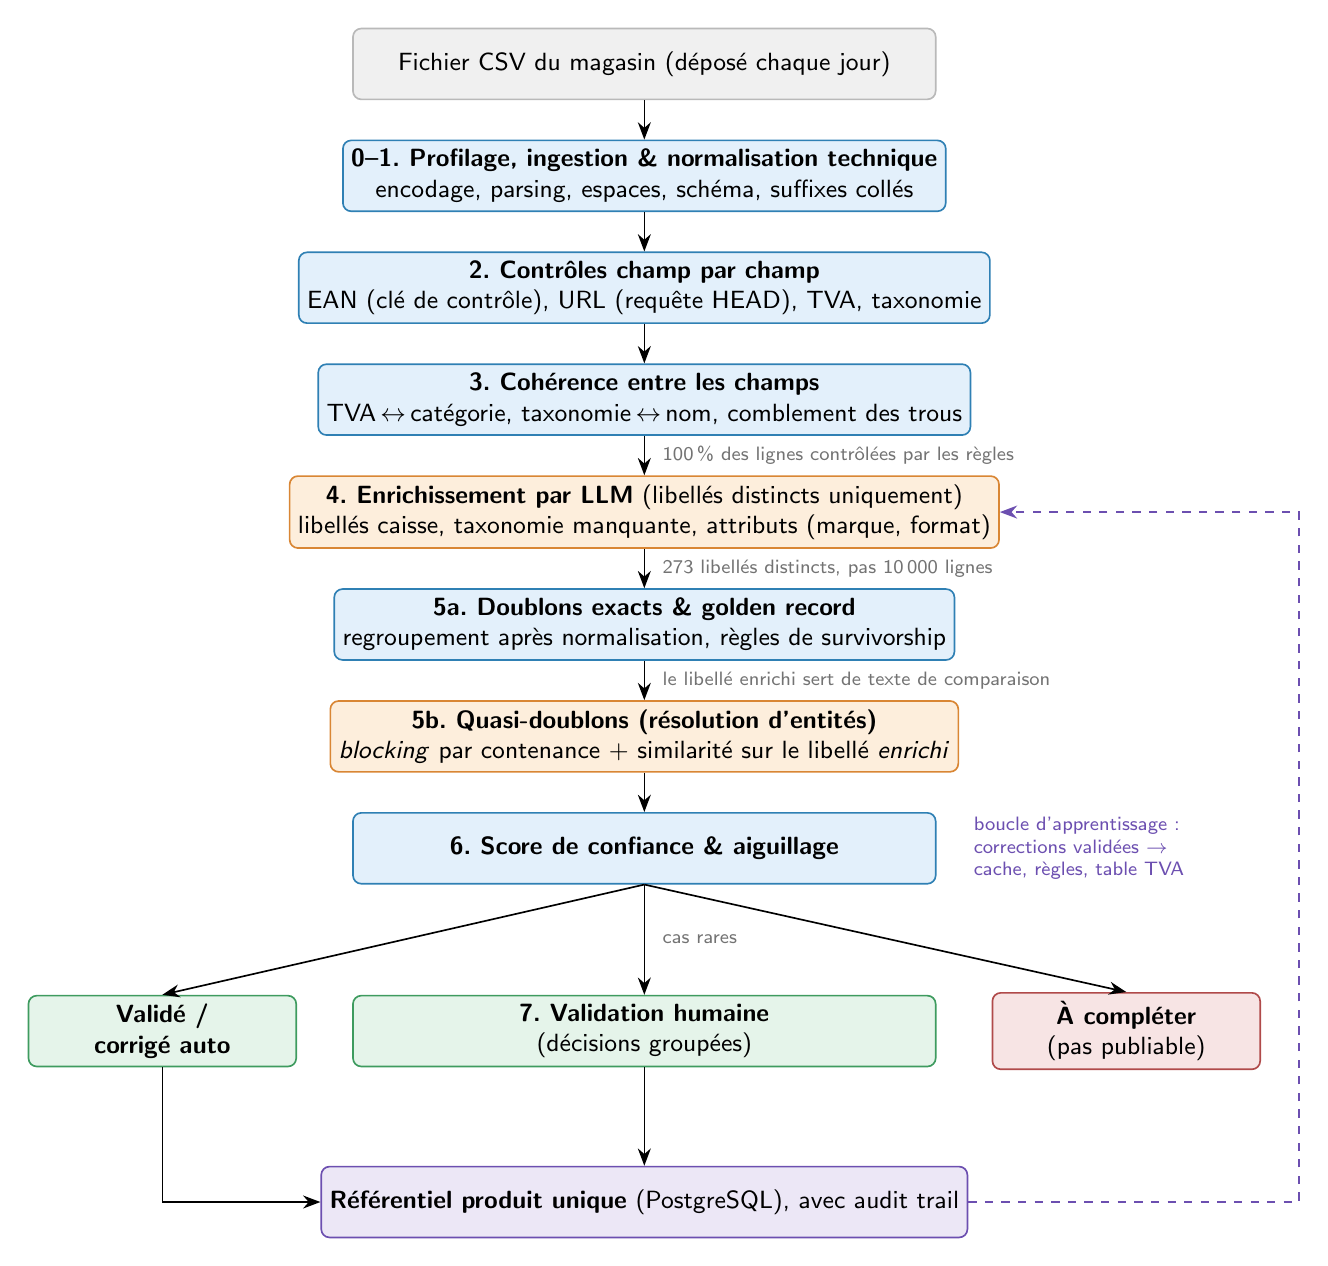
\begin{tikzpicture}[
  every node/.style={font=\small},
  box/.style={rectangle, rounded corners=3pt, draw, semithick,
              minimum width=7.4cm, minimum height=0.9cm, align=center, inner sep=3pt},
  det/.style={box, fill=detbg, draw=detln},
  sem/.style={box, fill=sembg, draw=semln},
  hum/.style={box, fill=humbg, draw=humln},
  src/.style={box, fill=gray!12, draw=gray!55},
  ref/.style={box, fill=refbg, draw=refln},
  rej/.style={box, fill=rejbg, draw=rejln, minimum width=3.4cm},
  okout/.style={box, fill=humbg, draw=humln, minimum width=3.4cm},
  ar/.style={-{Stealth[length=2.2mm]}, semithick},
  fb/.style={-{Stealth[length=2.2mm]}, semithick, dashed, draw=refln},
  vol/.style={font=\scriptsize, text=gray!90!black},
  node distance=0.5cm,
]

\node[src] (src) {Fichier CSV du magasin (déposé chaque jour)};
\node[det, below=of src] (ing) {\textbf{0--1. Profilage, ingestion \& normalisation technique}\\ encodage, parsing, espaces, schéma, suffixes collés};
\node[det, below=of ing] (val) {\textbf{2. Contrôles champ par champ}\\ EAN (clé de contrôle), URL (requête HEAD), TVA, taxonomie};
\node[det, below=of val] (coh) {\textbf{3. Cohérence entre les champs}\\ TVA\,$\leftrightarrow$\,catégorie, taxonomie\,$\leftrightarrow$\,nom, comblement des trous};
\node[sem, below=of coh] (llm) {\textbf{4. Enrichissement par LLM} (libellés distincts uniquement)\\ libellés caisse, taxonomie manquante, attributs (marque, format)};
\node[det, below=of llm] (dpx) {\textbf{5a. Doublons exacts \& golden record}\\ regroupement après normalisation, règles de survivorship};
\node[sem, below=of dpx] (dps) {\textbf{5b. Quasi-doublons (résolution d'entités)}\\ \emph{blocking} par contenance + similarité sur le libellé \emph{enrichi}};
\node[det, below=of dps] (sco) {\textbf{6. Score de confiance \& aiguillage}};

\node[hum, below=1.4cm of sco] (hitl) {\textbf{7. Validation humaine}\\ (décisions groupées)};
\node[okout, left=0.7cm of hitl] (auto) {\textbf{Validé /}\\\textbf{corrigé auto}};
\node[rej, right=0.7cm of hitl] (rej) {\textbf{À compléter}\\(pas publiable)};

\node[ref, below=1.25cm of hitl] (ref) {\textbf{Référentiel produit unique} (PostgreSQL), avec audit trail};

\foreach \a/\b in {src/ing, ing/val, val/coh}
  \draw[ar] (\a) -- (\b);

\draw[ar] (coh) -- (llm) node[midway, right=3pt, vol] {100\,\% des lignes contrôlées par les règles};
\draw[ar] (llm) -- (dpx) node[midway, right=3pt, vol] {273 libellés distincts, pas 10\,000 lignes};
\draw[ar] (dpx) -- (dps) node[midway, right=3pt, vol] {le libellé enrichi sert de texte de comparaison};
\draw[ar] (dps) -- (sco);
\draw[ar] (sco.south) -- (hitl.north) node[midway, right=3pt, vol] {cas rares};
\draw[ar] (sco.south) -- (auto.north);
\draw[ar] (sco.south) -- (rej.north);
\draw[ar] (auto.south) |- (ref.west);
\draw[ar] (hitl.south) -- (ref.north);

\draw[fb] (ref.east) -- ++(4.2,0) |- (llm.east);
\node[vol, align=left, anchor=west, text=refln] at ([xshift=0.35cm]sco.east)
  {boucle d'apprentissage~:\\ corrections validées $\to$\\ cache, règles, table TVA};

\end{tikzpicture}
\end{center}

En bleu, les règles. En orange, le sémantique. En vert, le seul endroit où un
humain intervient. La flèche en pointillés est la boucle de retour~: chaque correction validée est
mémorisée, donc le pipeline coûte moins cher chaque jour.

\textbf{Un point d'ordre, contre-intuitif et délibéré~: l'enrichissement par le LLM passe AVANT la
résolution des quasi-doublons.} On attendrait l'inverse. La raison est mesurée~: sur ce fichier,
27~\% des vraies paires de doublons tombent sous 0,45 de similarité textuelle brute. \guillemotleft{} DOLIP 1G
CPR \guillemotright{} et \guillemotleft{} DOLIPRANE 1 G \guillemotright{} ne se ressemblent pas assez pour être rapprochés. Une fois réécrits par
le LLM, les deux libellés convergent et le rapprochement flou les retrouve. Enrichir d'abord rend
donc la déduplication possible~; l'ordre inverse laisserait ces paires non détectées.

\section*{Dix minutes dans le fichier avant de concevoir}

L'énoncé n'exigeait pas de code, mais un pipeline se conçoit à partir des données réelles, pas
d'hypothèses. J'ai donc profilé le fichier fourni avant d'écrire quoi que ce
soit. Chaque constat ci-dessous vient du fichier, et chacun a changé une décision de conception.

\renewcommand{\arraystretch}{1.3}
\begin{tabularx}{\linewidth}{L{7.9cm} X}
\toprule
\textbf{Ce que le fichier contient vraiment} & \textbf{Ce que ça change dans le pipeline} \\
\midrule
\textbf{343} libellés distincts pour 10\,000 lignes, et \textbf{zéro doublon exact}~: aucun
\texttt{id\_produit} en double, aucun EAN non vide en double. Le cola s'écrit de \textbf{36}
façons (\guillemotleft{} COKA COLA ZERO 1 L \guillemotright{}, \guillemotleft{} COCACOLA Z 100CL \guillemotright{}, \guillemotleft{} COC COL ZER 1L \guillemotright{}...). &
Le sujet central est la résolution d'entités. L'EAN ne peut pas servir d'ancre~: chaque variante
porte un EAN différent. \\
\addlinespace
Les 10\,000 taux de TVA sont \textbf{tous légaux}. Et pourtant \textbf{394} sont incohérents avec
le produit~: whisky à 10, 5,5 ou 2,1~\%, \guillemotleft{} CAFE MLU 250G \guillemotright{} à 2,1~\%, \guillemotleft{} LESS. LIQUIDE 200CL \guillemotright{} à
2,1~\%. &
Le contrôle \guillemotleft{} taux légal \guillemotright{} capture zéro anomalie ici. Seul le croisement
catégorie\,$\to$\,taux attendu détecte les erreurs. \\
\addlinespace
\textbf{850} codes ne passent pas le checksum en l'état~: \textbf{386} redeviennent valides une
fois complétés à la bonne longueur, \textbf{331} une fois débarrassés de zéros de tête en trop,
et \textbf{133} n'ont que 3 à 5 chiffres. S'y ajoutent \textbf{1\,438} codes en préfixe GS1
interne, \textbf{1\,208} GTIN-14 (le carton, pas l'unité vendue) et \textbf{1\,300} vides. &
Un échec de checksum exige un diagnostic, pas un rejet~: réparable auto, code interne à router,
ou faux à signaler. \\
\addlinespace
\textbf{118} lignes en mojibake (\guillemotleft{} CAFÃ\textperthousand{} PUR ARAB 250 GR \guillemotright{}) et \textbf{153} lignes avec un
suffixe marketing collé sans espace (\guillemotleft{} WHISKY 40\%NEW FORMULA \guillemotright{}, \guillemotleft{} TOMATES GRAPPEFAMILY SIZE \guillemotright{},
\guillemotleft{} LESSIVE 2LORIGINE ITALIA \guillemotright{}). &
Mojibake réparé à l'ingestion~; suffixes détachés avant la similarité, sinon la déduplication
compare du bruit. \\
\addlinespace
\textbf{1\,278} lignes sans image exploitable~: 800 URLs vides, 400 pointant vers un chemin
\texttt{/missing/}, 78 malformées (\guillemotleft{} \texttt{not-a-url} \guillemotright{}). S'y ajoutent 86 URLs réparables
(\guillemotleft{} \texttt{htp://} \guillemotright{}, \guillemotleft{} \texttt{www.} \guillemotright{} sans schéma). &
Trois traitements~: réparable par règle, vérifiable par HEAD, irrécupérable à signaler. Près de
13~\% du catalogue invendable en l'état. \\
\addlinespace
\textbf{250} lignes ont un niveau 3 sans niveau 2, \textbf{400} ont une hiérarchie incomplète, et
\textbf{554} taxonomies contredisent le nom~: \guillemotleft{} PAMPERS BABY DRY 4 \guillemotright{} classé en LIQUIDE,
\guillemotleft{} WHISKY ECOSSAIS 70 CL \guillemotright{} en LIQUIDE, \guillemotleft{} CREME FRAICHE 30 20CL \guillemotright{} en NOISETTE CACAO. &
Le contrôle de hiérarchie ne suffit pas~: il faut croiser taxonomie et nom par mots-clés, et
envoyer ces cas en revue humaine. \\
\bottomrule
\end{tabularx}

\section*{Les étapes, une par une}

\textbf{0. Profilage.} Avant d'écrire la moindre règle, je mesure le fichier~: longueurs d'EAN,
taux de vide par colonne, libellés distincts, valeurs de TVA présentes. Dix minutes qui évitent de
construire sur des suppositions~; sur ce fichier, elles ont invalidé deux idées reçues (aucun
doublon exact à trouver, contrôle de liste TVA inutile) et produit le tableau ci-dessus.

\textbf{1. Ingestion et normalisation technique.} On remet le fichier d'aplomb. Forcer l'UTF-8 et
réparer le \emph{mojibake}, ces caractères cassés du type \guillemotleft{} CAFÃ\textperthousand{} PUR ARAB 250 GR \guillemotright{} qui
apparaissent quand un fichier UTF-8 est relu comme du Latin-1~; la réparation est mécanique et sans
risque. Neutraliser le BOM, un marqueur invisible qu'Excel ajoute parfois en tête de fichier et qui
pollue le nom de la première colonne. Lire le CSV proprement~: séparateurs, guillemets, retours à la
ligne au milieu d'un champ. Retirer les espaces superflus, vérifier que toutes les colonnes attendues
sont là.

Un piège mesuré à cette étape~: la réparation du mojibake crée une catégorie fantôme si on
s'arrête là. \guillemotleft{} ÉPICERIE SUCREE \guillemotright{} réparé ne correspond plus à \guillemotleft{} EPICERIE SUCREE \guillemotright{} du référentiel,
qui est sans accent. Il faut donc canonicaliser chaque niveau de taxonomie contre l'orthographe de
référence après réparation~; sans cela, 104 lignes se retrouvent dans une catégorie qui n'existe
pas. C'est le genre de défaut qu'aucune relecture de code ne trouve et qu'un compteur trouve tout
de suite.

Deuxième piège traité ici~: les mentions marketing collées au libellé sans espace
(\guillemotleft{} \texttt{FAMILY SIZE} \guillemotright{}, \guillemotleft{} \texttt{NEW FORMULA} \guillemotright{}, \guillemotleft{} \texttt{ORIGINE ITALIA} \guillemotright{}, collées en
\guillemotleft{} WHISKY 40\%NEW FORMULA \guillemotright{}). Si on ne les détache pas maintenant, elles fausseront le calcul de
similarité de l'étape 5b.

\textbf{2. Contrôles champ par champ.}
\begin{itemize}
  \item \textbf{ean}~: la clé de contrôle d'abord. Le dernier chiffre d'un EAN se calcule à partir
        des autres~; si le calcul ne retombe pas dessus, le code est faux, point. Mais un échec de
        checksum mérite un diagnostic, pas un rejet aveugle. Je distingue trois cas. Le code
        réparable par complétion~: \guillemotleft{} 789 \guillemotright{} complété en \guillemotleft{} 00000789 \guillemotright{} passe le checksum. Le code
        réparable par retrait~: \guillemotleft{} 003760000000130 \guillemotright{} débarrassé de ses zéros de tête redevient
        \guillemotleft{} 3760000000130 \guillemotright{}. Le code qui n'est pas un EAN~: \guillemotleft{} 31061 \guillemotright{}, trois à cinq chiffres, type
        PLU ou code balance~; et les préfixes GS1 20 à 29, réservés par le standard à l'usage
        interne (produits pesés, marques de distributeur), comme \guillemotleft{} 20000042 \guillemotright{}. Ceux-là sont
        légitimes, je les route comme codes internes au lieu de les \guillemotleft{} corriger \guillemotright{}.
  \item \textbf{url\_image}~: URL bien formée, puis une requête HEAD pour vérifier que l'image
        existe. HEAD demande au serveur les en-têtes de la ressource sans télécharger le fichier~:
        on obtient le statut (200 ou 404) et le type de contenu pour un coût minime. Certains
        serveurs refusent HEAD~; le repli est un GET limité au premier octet, mémorisé par domaine
        pour ne pas repayer le repli sur chaque URL. Sur 10\,000 lignes, ces appels partent en
        asynchrone avec une limite de concurrence et des timeouts, sinon la vérification prendrait
        des heures.

        Point important~: une image \textbf{non vérifiée} n'est pas une image \textbf{morte}. Le
        pipeline distingue les deux, et un produit dont l'image n'a pas été contrôlée n'est jamais
        déclaré publiable. Confondre les deux revient à publier des fiches à visuel cassé en
        croyant les avoir validées.
  \item \textbf{tva}~: le taux doit appartenir aux taux légaux français (2,1~; 5,5~; 10~; 20~\%).
        Ce contrôle est nécessaire mais très insuffisant~: ce fichier
        contient 100~\% de taux légaux et 394 erreurs de TVA, parce qu'un taux légal peut
        être appliqué au mauvais produit. Le vrai
        contrôle compare donc le taux au type de produit~; c'est le contrôle croisé de l'étape 3.
  \item \textbf{taxonomie}~: la hiérarchie doit tenir debout (pas de niveau 3 sans niveau 2), les
        valeurs doivent appartenir à la taxonomie de référence, et les variantes d'écriture d'une
        même catégorie sont rapprochées (\guillemotleft{} CRÈMERIE \guillemotright{} et \guillemotleft{} CREMERIE \guillemotright{} désignent la même chose).
\end{itemize}

Le tri complet des 10\,000 codes tient dans un schéma, et il totalise exactement 10\,000~: c'est
ce qui garantit qu'aucun code n'est compté deux fois ni oublié. Une fois le diagnostic posé, la
branche \guillemotleft{} réellement corrompu \guillemotright{} est vide.

\begin{center}
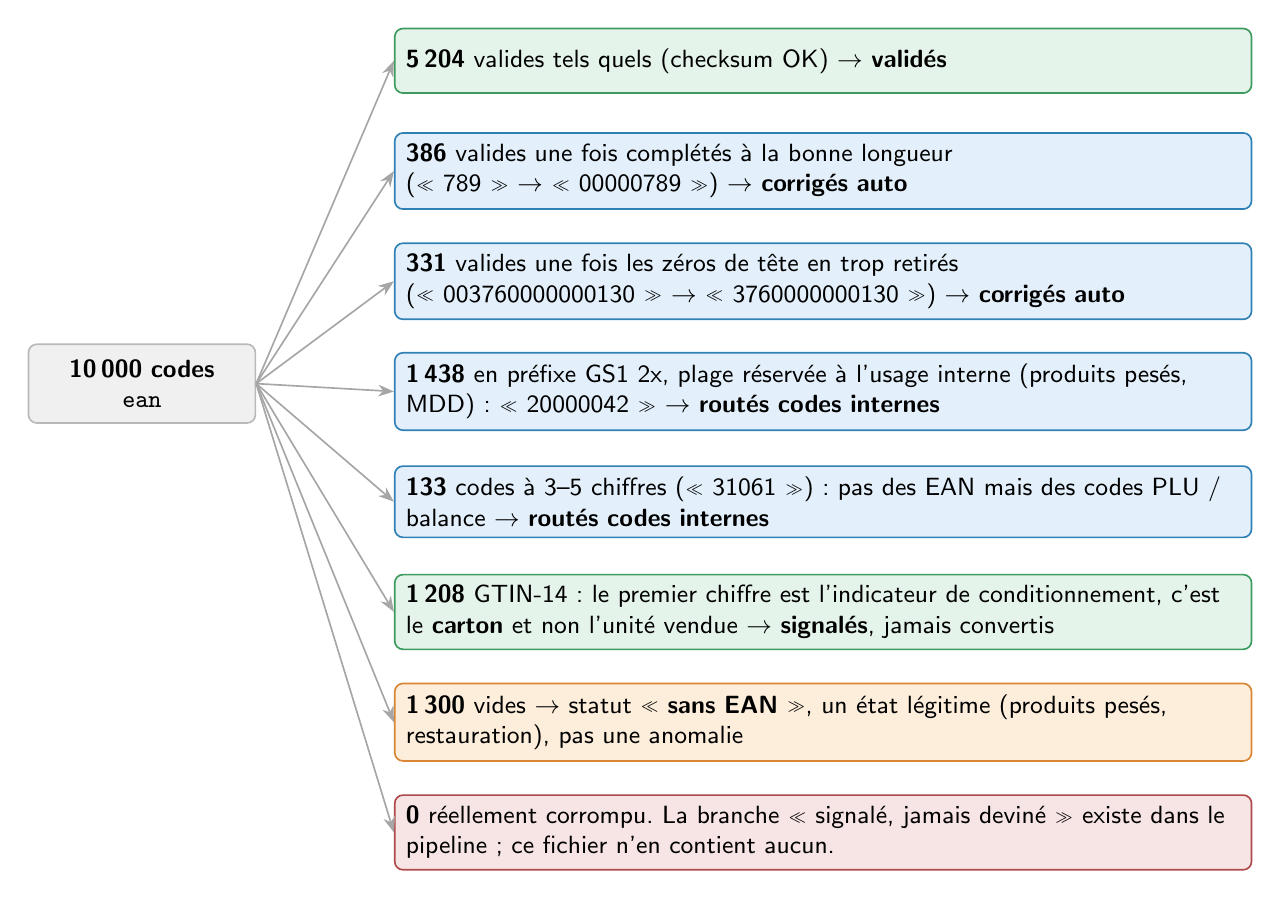
\begin{tikzpicture}[
  every node/.style={font=\small},
  leaf/.style={rectangle, rounded corners=3pt, draw, semithick, minimum height=0.82cm,
               text width=10.6cm, align=left, inner sep=4pt},
  root/.style={rectangle, rounded corners=3pt, draw=gray!55, fill=gray!12, semithick,
               minimum height=1cm, text width=2.6cm, align=center, inner sep=4pt},
  ar/.style={-{Stealth[length=2mm]}, semithick, gray!70},
]
\node[root] (r) at (0,0) {\textbf{10\,000 codes}\\ \texttt{ean}};
\node[leaf, fill=humbg, draw=humln, anchor=west] (a) at (3.2, 4.1)
  {\textbf{5\,204} valides tels quels (checksum OK) $\to$ \textbf{validés}};
\node[leaf, fill=detbg, draw=detln, anchor=west] (b) at (3.2, 2.7)
  {\textbf{386} valides une fois complétés à la bonne longueur\\
   (\guillemotleft{} 789 \guillemotright{} $\to$ \guillemotleft{} 00000789 \guillemotright{}) $\to$ \textbf{corrigés auto}};
\node[leaf, fill=detbg, draw=detln, anchor=west] (b2) at (3.2, 1.3)
  {\textbf{331} valides une fois les zéros de tête en trop retirés\\
   (\guillemotleft{} 003760000000130 \guillemotright{} $\to$ \guillemotleft{} 3760000000130 \guillemotright{}) $\to$ \textbf{corrigés auto}};
\node[leaf, fill=detbg, draw=detln, anchor=west] (c) at (3.2, -0.1)
  {\textbf{1\,438} en préfixe GS1 2x, plage réservée à l'usage interne
   (produits pesés, MDD)~: \guillemotleft{} 20000042 \guillemotright{} $\to$ \textbf{routés codes internes}};
\node[leaf, fill=detbg, draw=detln, anchor=west] (d) at (3.2, -1.5)
  {\textbf{133} codes à 3--5 chiffres (\guillemotleft{} 31061 \guillemotright{})~: pas des EAN mais des
   codes PLU / balance $\to$ \textbf{routés codes internes}};
\node[leaf, fill=humbg, draw=humln, anchor=west] (g) at (3.2, -2.9)
  {\textbf{1\,208} GTIN-14~: le premier chiffre est l'indicateur de conditionnement,
   c'est le \textbf{carton} et non l'unité vendue $\to$ \textbf{signalés}, jamais convertis};
\node[leaf, fill=sembg, draw=semln, anchor=west] (e) at (3.2, -4.3)
  {\textbf{1\,300} vides $\to$ statut \textbf{\guillemotleft{} sans EAN \guillemotright{}}, un état légitime
   (produits pesés, restauration), pas une anomalie};
\node[leaf, fill=rejbg, draw=rejln, anchor=west] (f) at (3.2, -5.7)
  {\textbf{0} réellement corrompu. La branche \guillemotleft{} signalé, jamais deviné \guillemotright{} existe dans le
   pipeline~; ce fichier n'en contient aucun.};
\foreach \x in {a,b,b2,c,d,g,e,f} \draw[ar] (r.east) -- (\x.west);
\end{tikzpicture}
\end{center}

\textbf{3. Cohérence entre les champs.} On croise les champs entre eux. La taxonomie est-elle
compatible avec le nom~? Un \guillemotleft{} WHISKY ECOSSAIS 70 CL \guillemotright{} classé en LIQUIDE est une contradiction
franche, détectable par une simple règle de mots-clés~; le fichier en contient 554.

Pour la TVA, une table de correspondance catégorie vers taux attendu détecte
l'essentiel~: alcools et entretien à 20~\%, alimentaire courant à 5,5~\%, médicaments remboursables
à 2,1~\%. Elle relève 394 lignes. Dans tous les cas on signale la contradiction, on ne la corrige
pas en douce.

Une précaution non évidente~: cette règle n'est appliquée que si la taxonomie ne contredit pas
déjà le nom du produit. Sans ce garde-fou, une ligne mal classée déclenche deux anomalies pour un
seul défaut, et le décompte passe de 394 à 615 erreurs de TVA apparentes. Compter deux fois le même
problème n'est pas neutre~: cela gonfle artificiellement la charge de revue humaine.

\textbf{Sur les référentiels externes.} L'idée de croiser l'EAN avec une base publique (GS1, Open
Food Facts) est la bonne en production. Je l'ai testée sur ce fichier avant de l'implémenter, et le
résultat commande de ne pas le faire ici~: sur six EAN valides tirés du fichier, un seul existe dans
Open Food Facts, et c'est une \textbf{fausse correspondance}. Le code 3760000000024 vaut \guillemotleft{} TOMATES
GRAPPE \guillemotright{} dans le fichier et \guillemotleft{} Guimauve Chocolat Lait \guillemotright{} dans la base publique. Les EAN de cet
échantillon sont synthétiques~; un croisement externe ne trouverait rien dans 99~\% des cas et,
dans le cas restant, signalerait comme anomalie une ligne correcte, voire \guillemotleft{} corrigerait \guillemotright{} des
tomates en guimauve. C'est un branchement qui a sa place le jour où le catalogue porte de vrais
codes-barres, pas avant. Je préfère un pipeline qui ne fait pas semblant.

\textbf{4. Enrichissement par LLM.} C'est là qu'il apporte le plus~: réécrire les libellés caisse
du fichier (\guillemotleft{} CAFE MLU 250G \guillemotright{} devient \guillemotleft{} Café moulu 250 g \guillemotright{}, \guillemotleft{} CRÈME FR. EPAISSE 20 CL \guillemotright{} devient
\guillemotleft{} Crème fraîche épaisse 20 cl \guillemotright{}), compléter une taxonomie manquante à
partir du nom, extraire des attributs structurés (marque, contenance, unité).

Trois précautions dans la façon de l'appeler. Une sortie contrainte en JSON
avec un schéma imposé, pour que la réponse soit exploitable par la machine et jamais du texte
libre. La taxonomie de référence fournie dans le prompt, pour qu'il choisisse parmi les catégories
existantes au lieu d'en inventer. Un score de confiance demandé en retour, qui alimente l'étape 6~;
sous le seuil, la proposition existe mais n'est pas appliquée, et le cas part en revue.

Et une règle d'économie~: je lui envoie les libellés \emph{distincts}, pas les lignes. Sur ce
fichier, 273 au lieu de 10\,000, soit un facteur 37. Les réponses sont mises en cache
\textbf{libellé par libellé}, et non par lot~: un lot de 25 libellés cesse d'être réutilisable dès
qu'un seul produit apparaît ou disparaît, puisque la composition de tous les lots suivants se
décale. Mesuré sur les 273 libellés, avec 5~\% de nouveautés au dépôt suivant~: une clé par lot
refacture 100~\% du catalogue, une clé par libellé n'en refacture que 5~\%.

\textbf{5. Doublons, ou plutôt résolution d'entités.} Les doublons exacts se
règlent par comparaison directe une fois les données normalisées~; sans normalisation préalable, un
espace ou un zéro perdu suffit à rater l'égalité. Je garde cette étape parce qu'elle sert dans la
vraie vie, mais je note que sur ce fichier précis elle ne capture rien~: le profilage montre zéro
doublon exact. Toute la difficulté a été déplacée vers les quasi-doublons~: reconnaître que
\guillemotleft{} COKA COLA ZERO 1 L \guillemotright{}, \guillemotleft{} COCACOLA Z 100CL \guillemotright{} et \guillemotleft{} COC COL ZER 1L \guillemotright{}, trois des 23 écritures du même
produit dans le fichier, désignent une seule référence. Je mène cette résolution en deux temps~:
\begin{itemize}
  \item \textbf{blocking}~: ne comparer que les fiches d'une même classe (catégorie feuille +
        contenance). Comparer 273 fiches deux à deux ferait 37\,128 paires~; le blocking ramène
        ça à 2\,507 comparaisons utiles. La contenance est une barrière
        \emph{dure}, mais elle porte sur le VOLUME, pas sur les caractères~: le
        magasin écrit la même bouteille \guillemotleft{} 1 L \guillemotright{},
        \guillemotleft{} 100CL \guillemotright{} ou \guillemotleft{} 0.7L \guillemotright{} selon la caisse, et les trois
        doivent se rencontrer. En revanche
        \guillemotleft{} COCA COLA ZERO 1L \guillemotright{} et un même produit en 33~cl se ressemblent énormément
        et sont deux références différentes~;
  \item \textbf{similarité textuelle} (RapidFuzz) sur le libellé \emph{enrichi par le LLM}, pas
        sur le libellé brut. Au-dessus de 0,86 on fusionne, en dessous de 0,72 on sépare~; entre
        les deux, on ne fusionne pas et le doublon reste. C'est délibéré~: une fusion à tort est
        invisible et irréversible, un doublon restant se voit.
\end{itemize}

\textbf{Pourquoi pas d'embeddings.} C'était mon intention de départ. La mesure l'a écartée~: 27~\%
des vraies paires tombent sous 0,45 de similarité brute, ce qui justifiait un modèle sémantique,
mais le LLM voit déjà chaque libellé distinct exactement une fois et comble ce même fossé sans
appel supplémentaire. Ajouter \texttt{sentence-transformers} aurait coûté environ 2~Go de
dépendances (via \texttt{torch}) sur un serveur qui en a 3,8, pour un gain déjà obtenu. RapidFuzz
pèse environ 1~Mo. La bonne raison de ne pas ajouter une brique, c'est qu'une autre fait déjà le
travail.

\begin{center}
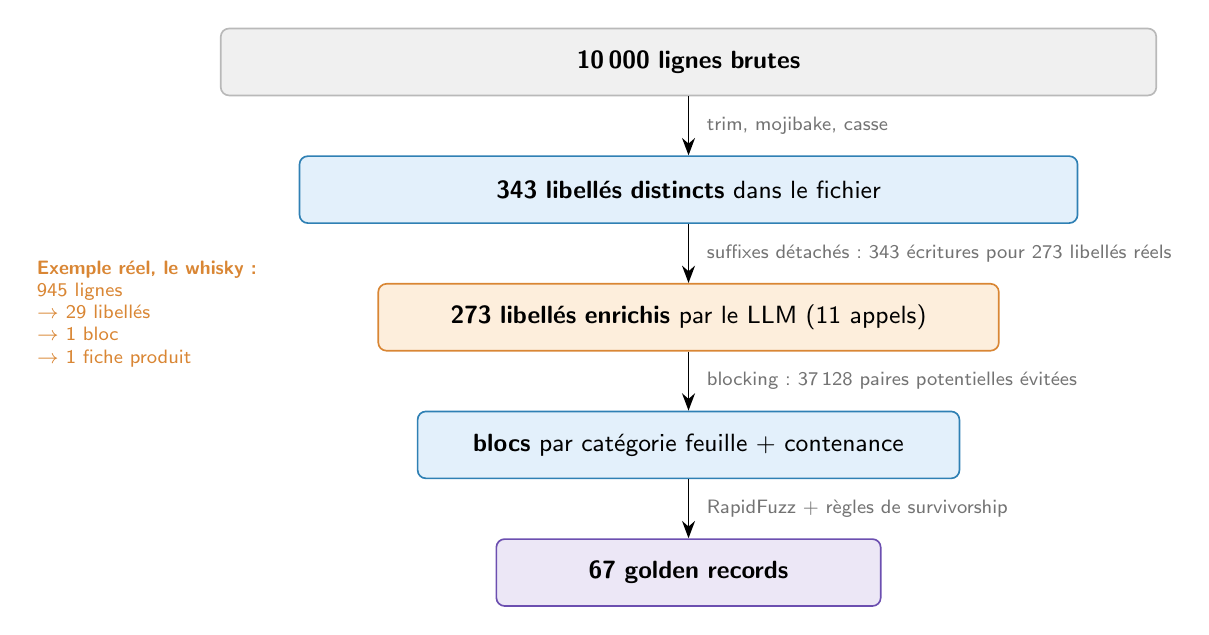
\begin{tikzpicture}[
  every node/.style={font=\small},
  fun/.style={rectangle, rounded corners=3pt, draw, semithick, minimum height=0.85cm,
              align=center, inner sep=4pt},
  ar/.style={-{Stealth[length=2.2mm]}, semithick},
  lab/.style={font=\scriptsize, text=gray!90!black, right=3pt},
  side/.style={font=\scriptsize, text=semln, align=left},
]
\node[fun, fill=gray!12, draw=gray!55, text width=11.6cm] (n1) at (0,0)
  {\textbf{10\,000 lignes brutes}};
\node[fun, fill=detbg, draw=detln, text width=9.6cm, below=0.75cm of n1] (n2)
  {\textbf{343 libellés distincts} dans le fichier};
\node[fun, fill=sembg, draw=semln, text width=7.6cm, below=0.75cm of n2] (n3)
  {\textbf{273 libellés enrichis} par le LLM (11 appels)};
\node[fun, fill=detbg, draw=detln, text width=6.6cm, below=0.75cm of n3] (n4)
  {\textbf{blocs} par catégorie feuille + contenance};
\node[fun, fill=refbg, draw=refln, text width=4.6cm, below=0.75cm of n4] (n5)
  {\textbf{67 golden records}};

\draw[ar] (n1) -- (n2) node[lab, midway] {trim, mojibake, casse};
\draw[ar] (n2) -- (n3) node[lab, midway] {suffixes détachés~: 343 écritures pour 273 libellés réels};
\draw[ar] (n3) -- (n4) node[lab, midway] {blocking~: 37\,128 paires potentielles évitées};
\draw[ar] (n4) -- (n5) node[lab, midway] {RapidFuzz + règles de survivorship};

\node[side, anchor=west] at (-8.4,-3.2)
  {\textbf{Exemple réel, le whisky~:}\\ 945 lignes\\ $\to$ 29 libellés\\ $\to$ 1 bloc\\ $\to$ 1 fiche produit};
\end{tikzpicture}
\end{center}

Les 71 fiches sont le chiffre mesuré sans l'étage LLM (exécution hors réseau). Avec l'enrichissement
actif, le rapprochement flou opère sur des libellés convergents et le nombre descend nettement~; je
ne donne pas de chiffre que je n'ai pas mesuré sur le fichier complet.

Une fois un groupe de doublons confirmé, il faut construire la fiche unique, ce que le métier
appelle le \emph{golden record}, avec des règles de \emph{survivorship} écrites noir sur blanc~:
quelle valeur survit à la fusion. Je prends le libellé le plus complet, l'EAN qui passe le
checksum, l'URL d'image qui répond, la taxonomie la plus profonde. Un désaccord de TVA entre fiches
fusionnées ne se tranche jamais d'autorité~: il marque le groupe en conflit et l'envoie en revue.
Fusionner sans règles écrites, c'est perdre de l'information sans s'en rendre compte.

\textbf{Et les 10\,000 lignes ne disparaissent pas.} Le référentiel compte quelques dizaines de
fiches, mais chaque ligne source garde son rattachement~: son identifiant tel que le magasin
l'écrit, son libellé d'origine, et la fiche qui la représente. C'est indispensable~: le système du
magasin continue de parler avec ses identifiants à lui, et \guillemotleft{} stock de tel code = 12 \guillemotright{} doit pouvoir
être relié au bon produit. Fusionner sans conserver ce fil reviendrait à couper le lien avec le
magasin.

\textbf{6. Score et aiguillage.} Chaque produit ressort avec un statut~: validé, corrigé
automatiquement, à revoir, ou à compléter. Le seuil dépend du champ. J'accepte automatiquement une
reformulation de libellé à haute confiance~; je n'accepte jamais un changement de TVA sans
validation, quel que soit le score.

\textbf{7. Validation humaine, en décisions groupées.} On n'y envoie que le strict nécessaire~:
propositions du LLM peu sûres, contradictions non résolues, création d'une nouvelle catégorie, et
tout ce qui touche à la TVA.

Grâce à la résolution d'entités, l'humain ne relit pas des centaines de lignes une par une~: il
tranche une poignée de décisions groupées, du type \guillemotleft{} les 32 lignes de ce whisky ont une TVA
différente de 20~\%~: appliquer 20~\% partout~? \guillemotright{}. Une petite interface de revue suffit.

Et chaque décision validée repart dans la boucle
du schéma~: elle enrichit le cache, les règles et la table catégorie vers TVA, donc la même
question n'est jamais posée deux fois.

\section*{La vie d'un produit dans le pipeline}

Pour rendre tout ça concret, je suis un produit réel du fichier de bout en bout~: le whisky.
\textbf{945 lignes} du fichier décrivent en réalité cette seule bouteille, sous \textbf{29
libellés} différents. Les quatre plus fréquents~: \guillemotleft{} WHISKY ECOSSAIS 70 CL \guillemotright{} (229 lignes),
\guillemotleft{} WHISKY 40 70CL \guillemotright{} (223), \guillemotleft{} WHISKY BTL 0.7L \guillemotright{} (215), \guillemotleft{} WHISKY 40\% \guillemotright{} (206).

\begin{center}
\fcolorbox{detln}{gray!5}{\begin{minipage}{0.95\linewidth}\small
\textbf{Étape 1.} \guillemotleft{} WHISKY 40\%NEW FORMULA \guillemotright{} perd son suffixe collé et redevient \guillemotleft{} WHISKY 40\% \guillemotright{}.
Les EAN portant des zéros de tête en trop sont recadrés et repassent le checksum.

\textbf{Étape 2.} Sur les 945 lignes~: 127 EAN vides, 93 URLs vides et 44 images pointant vers
\texttt{/missing/} sont signalés. Le taux de TVA de chaque ligne est légal, donc ce contrôle-là
ne dit rien.

\textbf{Étape 3.} La table catégorie\,$\to$\,taux repère 32 lignes hors des 20~\% attendus pour un
alcool~: 15 à 10~\%, 9 à 5,5~\%, 8 à 2,1~\%. Le contrôle taxonomie\,$\leftrightarrow$\,nom repère
9 lignes classées en ENTRETIEN et 8 en MEDICAMENTS. Tout est signalé, rien n'est corrigé en douce.

\textbf{Étape 4.} Le LLM ne voit que les 29 libellés distincts, pas les 945 lignes, et propose le
libellé propre \guillemotleft{} Whisky écossais 40\% 70 cl \guillemotright{}.

\textbf{Étape 5b.} Le blocking regroupe les 29 libellés en un seul bloc, la similarité sur les
libellés enrichis confirme qu'ils désignent le même produit. Le golden record retient le libellé le
plus complet, un EAN qui passe le checksum, une image qui répond, et la taxonomie majoritaire
BOISSONS (835 lignes sur 945).

\textbf{Étape 7.} L'humain reçoit \textbf{une seule décision groupée}~: \guillemotleft{} 32 lignes de ce produit
ont une TVA différente de 20~\%~: appliquer 20~\% partout~? \guillemotright{}. Un clic, la correction s'applique,
l'audit trail garde la trace, et la règle entre dans la table catégorie\,$\to$\,TVA~: demain, la
question ne sera plus posée.

\textbf{Bilan~:} 945 lignes en entrée, 1 fiche produit en sortie, 1 décision humaine, et 945
rattachements conservés vers les identifiants du magasin.
\end{minipage}}
\end{center}

\section*{Ce qu'on corrige seul, ce qu'on signale}

\renewcommand{\arraystretch}{1.25}
\begin{tabularx}{\linewidth}{L{5.6cm} L{4.0cm} X}
\toprule
\textbf{Anomalie} & \textbf{Traitement} & \textbf{Correction automatique ?} \\
\midrule
Encodage cassé (mojibake), BOM, espaces & Règles & Oui, déterministe \\
Accent réparé absent du référentiel & Règles (canonicalisation) & Oui, contre l'orthographe de référence \\
URL au schéma tronqué (\texttt{htp://}, \texttt{www.}) & Règles & Oui~; les URLs mortes sont signalées \\
Image non vérifiée & Règles & Non~: distinguée d'une image morte, bloque la publication \\
EAN à compléter ou à dézéroter & Règles (re-checksum) & Oui, si le code redevient valide \\
Code court type PLU ou préfixe GS1 interne & Règles & Routé comme code interne, pas \guillemotleft{} corrigé \guillemotright{} \\
EAN qui rate le checksum sans être réparable & Règles & Signalé, jamais deviné \\
TVA hors liste légale & Règles & Signalé \\
TVA légale mais incohérente avec le produit & Règles croisées + humain & Signalé, jamais fixé seul \\
Doublons exacts & Règles & Oui, après normalisation \\
Quasi-doublons & Blocking + RapidFuzz sur libellé enrichi & Fusionné au-dessus du seuil haut~; la zone grise reste séparée \\
Libellé caisse abrégé & LLM & Oui, si le score dépasse le seuil \\
Taxonomie manquante & LLM & Proposé \\
Taxonomie contredisant le nom & Règles + humain & Signalé \\
\bottomrule
\end{tabularx}

\section*{Où le LLM aide, où il ne décide pas}

Ma règle tient en une phrase~: le LLM propose, il ne décide jamais seul sur un champ à risque. Le
meilleur exemple est la TVA~: un mauvais taux a des conséquences fiscales pour le commerçant.
Dans l'implémentation, je suis allé plus loin que \guillemotleft{} il ne décide pas \guillemotright{}~: \textbf{le champ TVA n'est
pas soumis au modèle du tout}. Le prompt le lui interdit explicitement. Un modèle ne peut pas se
tromper sur une valeur qu'on ne lui montre pas.

Les contradictions entre champs expliquent pourquoi la revue humaine n'est pas un aveu d'échec
de l'automatisation. Quand le fichier dit
\guillemotleft{} PAMPERS BABY DRY 4 \guillemotright{} classé en LIQUIDE, la machine sait qu'un des deux champs ment,
mais trancher lequel exige une information qu'elle n'a pas~: le produit physique réel. Soit le nom
est juste et c'est la catégorie qui est fausse, soit l'inverse, et les deux corrections sont
opposées.

Le LLM dira \guillemotleft{} couches \guillemotright{} avec 90~\% de confiance, et il aura probablement raison. Mais
\guillemotleft{} probablement \guillemotright{} ne suffit pas ici, parce que l'erreur ne coûte pas pareil dans les deux sens.
Prenez \guillemotleft{} WHISKY ECOSSAIS 70 CL \guillemotright{} classé en LIQUIDE~: si on fait confiance au nom et qu'on reclasse
en SPIRITUEUX, on déclenche la TVA à 20~\%, les restrictions de vente d'alcool de la plateforme et
la vérification d'âge à la livraison~; si c'était en réalité un produit d'entretien au libellé
erroné, on vient d'imposer un contrôle d'identité pour acheter du détergent. Et dans l'autre sens,
garder LIQUIDE alors que c'est vraiment du whisky, c'est vendre de l'alcool sans restriction d'âge
et à la mauvaise TVA, une infraction réglementaire et fiscale chez le client.

Quand les deux issues d'un pari sont
aussi asymétriques, on ne parie pas~: le LLM propose sa correction avec son score, et un humain,
qui tranche ce genre de cas en une seconde, valide ou infirme. Grâce aux décisions groupées, ce
verrou coûte un clic, pas une relecture.

Une nuance pour finir~: cette frontière n'est pas figée,
elle dépend des preuves disponibles. Le jour où un référentiel externe confirme l'EAN et que le nom
concorde, deux sources contre une, la taxonomie isolée pourra se corriger automatiquement.
Autrement dit, plus les référentiels sont riches, plus de cas basculent de l'humain vers les
règles. Vers les règles, pas vers le LLM~: interroger une base est un traitement déterministe, et
demander à un LLM un lien EAN\,$\leftrightarrow$\,produit de mémoire serait le cas d'école de
l'hallucination. Ce qui reste à l'humain quoi qu'il arrive, ce sont les décisions qui engagent~:
la TVA et la création de catégories.

Et il y a des
tâches où le LLM serait un contre-emploi~: vérifier une clé de contrôle d'EAN est de
l'arithmétique, pas de la compréhension. Une règle le fait parfaitement, gratuitement, sans risque
d'invention. Bien positionner un LLM, c'est autant savoir où il n'a rien à faire que là où il
excelle.

\begin{tabularx}{\linewidth}{X X}
\toprule
\textbf{Le LLM est utile pour} & \textbf{Le LLM ne tranche pas seul} \\
\midrule
Nettoyer les libellés abrégés & Fixer un taux de TVA (champ non soumis) \\
Compléter une taxonomie manquante & Régler une incohérence taxonomie\,$\leftrightarrow$\,nom \\
Extraire des attributs (marque, format) & Créer une nouvelle catégorie \\
Rendre les quasi-doublons comparables & Valider un checksum (rôle des règles) \\
 & Tout cas où le score est trop bas \\
\bottomrule
\end{tabularx}

\section*{Ce que coûte l'étage LLM, et pourquoi c'est mesuré}

Un pipeline qui appelle un LLM sans montrer ce qu'il coûte est un pipeline dont personne ne peut
arbitrer l'usage. L'interface affiche donc, pour chaque traitement~: le modèle utilisé, son tarif,
le nombre d'appels réels, le nombre de libellés servis par le cache, les jetons consommés et le
coût en dollars, décomposé entre entrée, sortie et cache.

Trois leviers, dans l'ordre de leur effet mesuré~:
\begin{itemize}
  \item \textbf{la déduplication avant appel}~: 273 libellés au lieu de 10\,000 lignes, facteur 37~;
  \item \textbf{le cache par libellé}~: au deuxième dépôt du même magasin, seuls les libellés jamais
        vus sont facturés. Mesuré sur ce fichier avec 5~\% de nouveautés~: 5~\% du catalogue
        refacturé, contre 100~\% avec un cache par lot~;
  \item \textbf{le mode de traitement}~: l'API asynchrone d'Anthropic facture moitié prix les
        requêtes dont la réponse peut attendre. Le traitement nocturne planifié n'a aucune raison
        de payer la vitesse~; un dépôt fait à la main devant une barre de progression, si. Le choix
        est offert au dépôt, avec son prix affiché.
\end{itemize}

Un plafond de dépense cumulé coupe l'appel au LLM au-delà d'un montant fixé, et le reste du
pipeline continue de tourner~: un catalogue à moitié enrichi vaut mieux qu'un traitement en échec.

\section*{Pour conclure sur le périmètre demandé}

L'exercice porte sur un seul fichier magasin. À l'échelle réelle d'ULTY, avec des
centaines de magasins, le vrai enjeu devient de reconnaître qu'un même produit vu chez plusieurs
enseignes est une seule entité. La logique décrite ici ne change pas, mais la résolution d'entités
devient centrale~: l'EAN sert d'ancre quand il est fiable, et le sémantique (libellé normalisé,
attributs extraits) prend le relais quand il ne l'est pas~: codes internes, EAN manquants ou
erronés, exactement les cas que le pipeline aura appris à reconnaître.

C'est aussi à cette échelle que le cache prend tout son sens~: \guillemotleft{} COCA COLA ZERO 1L \guillemotright{} chez deux
enseignes différentes, c'est le même travail d'enrichissement. Payé une fois.

\vspace{0.5em}
\end{document}
